\documentclass[preprint,12pt]{elsarticle}
\usepackage[UTF8,scheme=plain,fontset=fandol]{ctex}
\usepackage{amsmath,amssymb,bm}
\usepackage{booktabs,multirow,threeparttable}
\usepackage{graphicx,subcaption}
\usepackage{xcolor,hyperref,lineno,enumitem,placeins}
\graphicspath{{../figures/}}
\hypersetup{colorlinks=true,linkcolor=blue!50!black,citecolor=blue!50!black,urlcolor=blue!60!black}
\emergencystretch=2em
\journal{Transportation Research Part C}
\renewcommand{\figurename}{图}
\renewcommand{\tablename}{表}

\begin{document}
\begin{frontmatter}

\title{面向全生命周期成本与油电混行能耗的高速公路三维线形数据驱动协同优化}

\author[aff1]{匿名作者}
\affiliation[aff1]{organization={双盲审稿匿名单位},city={匿名},country={中国}}

\begin{abstract}
高速公路的平面与纵断面决策共同决定地形扰动、桥隧工程、建设支出和长期车辆运行。本文构建空间显式双目标框架，融合14,018个GNSS中线点、去除既有道路影响后的准天然数字高程模型（DEM）以及OpenStreetMap（OSM）交通和水系要素。候选平面由50个正弦模态描述，纵断面由1个起点高程变量和224个坡段变量描述。全生命周期成本包含占地、基本工程、结构、土方和养护；第二目标将30年油电混行车流的燃油与电耗货币化。线形与空间障碍相交时触发跨越桥，连通山体区触发生态隧道，改进水母搜索算法（IJS）用于近似成本—能耗前沿；随后依次执行可行性、规划预算、非支配和熵权折中筛选。

广州北环高速22.46 km案例中，可行联合方案将成本由26.4061亿元降至24.2239亿元（8.26\%），将货币化能耗由13.9460亿元降至13.4766亿元（3.37\%）；线路缩短98.3 m，以401.0 m最小半径满足400 m要求，存储罚值为0。结构费减少2.6141亿元，抵消了0.4550亿元的土方增加。两阶段方案虽有更低原始目标，但因最小半径仅397.1 m而不可行。同代数消融与算法对比中，IJS的观测均值最低，但函数评价次数不等，不能据此声称等预算优势。纵断面端点未锚定且能耗仅按单向计算，因此结论仅属于走廊规划层面的计算证据。
\end{abstract}

\begin{keyword}
高速公路线形优化 \sep 数字高程模型 \sep OpenStreetMap \sep 改进水母搜索算法 \sep 全生命周期成本 \sep 车流能耗 \sep 平纵协同
\end{keyword}
\end{frontmatter}

\linenumbers

\section{引言}

高速公路线形是影响长期建设与运营的前期决策。线位横移会改变所穿越的地形、占地、桥隧需求、土方平衡和车辆所经历的坡度；平面缩短可能恶化纵断面，绕避山体可能增加交叉工程，而局部低成本方案也可能违反几何约束。因此，线形选择不是平面与纵断面的分别拟合，而是受空间数据、工程约束和竞争目标共同支配的三维优化问题。

经典研究较早证明了平纵同步优化的必要性\cite{chew1989,jong2003}。随后，GIS走廊、混合整数模型、环境目标与偏好驱动搜索得到发展\cite{kang2012,mondal2015,hirpa2016,vazquez2018,akhmet2022}。近年研究进一步结合BIM、强化学习、采样式规划和混合元启发式方法\cite{han2023,he2023,alhadad2024,pu2024,pu2026}。然而，将异构空间信息一致地转化为可追踪工程量仍是主要困难\cite{songreview2023}。

本文聚焦三个缺口。第一，单一中线地面高程无法反映平面横移后实际遇到的地形。第二，固定桥隧长度可能使优化器利用计价假设，而不是发现新的工程走廊。第三，高维平纵搜索既需要全局探索和局部细化，也必须在细空间尺度上核验可行性。

本文贡献包括：

\begin{enumerate}[leftmargin=*,label=(\arabic*)]
\item 建立候选平面与准天然DEM、OSM交叉要素联动的数字走廊；
\item 构建包含几何触发桥梁、生态隧道和土方—结构替代的可审计全生命周期模型；
\item 建立275变量的平纵协同表示，并在熵权决策前执行可行性、预算和非支配筛选；
\item 对IJS工程方案、联合—两阶段对照、同代数机制消融、多算法比较和重优化敏感性结果进行边界清晰的解释。
\end{enumerate}

图\ref{fig:overview_zh}概括整体流程。全文数值严格固定于Git提交\texttt{c1327df}，完整哈希记录于源文件清单；不混入后续固定纵断面端点或建筑密度版本的结果。

\begin{figure}[!htbp]
\centering
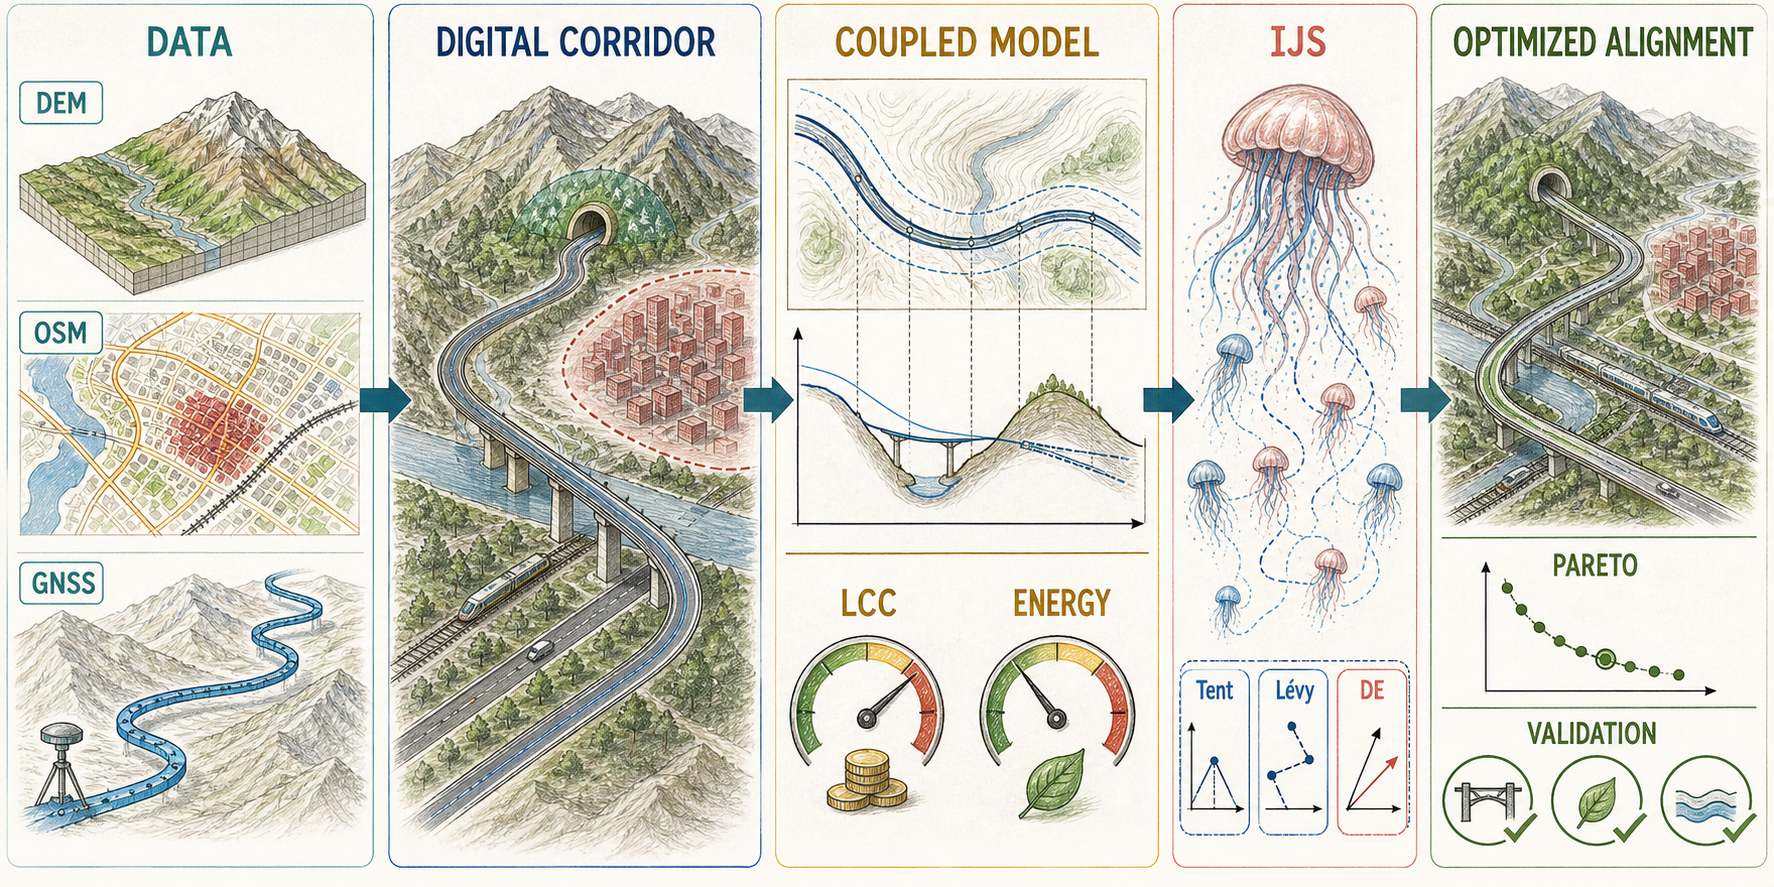
\includegraphics[width=\textwidth]{method_overview_handdrawn.png}
\caption{从空间数据、协同目标到IJS搜索与折中决策的流程。图中的建筑仅作走廊情境表达；固定版本使用DEM和OSM交通/水系交叉，不包含建筑密度约束。}
\label{fig:overview_zh}
\end{figure}

\section{相关研究}

\subsection{三维线形优化}

平纵同步模型可以避免顺序设计造成的不一致\cite{chew1989,jong2003}。GIS方法扩展了可行走廊并引入环境图层\cite{kang2012,davey2017}；走廊约束和数学规划提高了模型可解性\cite{mondal2015,akhmet2022}；双目标公路与铁路模型进一步考虑成本、灾害和生态影响\cite{hirpa2016,zhang2020,song2022}。本文重点是建立候选坐标到地形、交叉、工程量和目标值的可追踪映射。

\subsection{全生命周期成本与车流能耗}

成本分类沿用林坤锐\cite{lin2025}的数学基础，包括占地、桥隧、基本工程、养护和土方。道路距离、坡度和曲率共同影响车辆能耗\cite{llopis2019}；电动车能耗还与传动效率和再生制动有关\cite{dimartino2022}。本文先分别计算燃油和电耗，再按统一30年期限货币化。该处理提供一致决策尺度，但不能替代完整环境评价。

\subsection{算法与折中决策}

NSGA-II是常用多目标基线\cite{deb2002}。水母搜索（JS）通过洋流运动和主动/被动运动更新个体\cite{chou2021}。IJS加入Tent初始化、L\'evy探索和差分进化（DE）细化\cite{storn1997}。基于Shannon信息的熵权法\cite{shannon1948}有两个相互独立的用途：从共同初始种群确定标量搜索权重，以及在可行非支配集合中选择折中方案。

\section{数据驱动数学模型}\label{sec:model_zh}

\subsection{案例走廊与空间数据}

案例为广州北环高速浔峰洲—黄村段，双向六车道。现状M-A中线包含14,018个GNSS点，在共同评价器下长度为22.4618 km。所有候选线固定平面起终点。

地形来自60幅AWS Terrain Tiles，缩放等级14，像元约8.8 m\cite{awsterrain}。为减弱既有道路表面对地面的影响，先删除现状线两侧$\pm60$ m范围，再由相邻地形插值得到准天然DEM。经常数高程基准修正后，该表面与实测中线高程的相关系数为0.915。OSM提供道路、铁路与水系\cite{haklay2008,osmlicense}；剔除北环自身及伴行设施后，存储障碍物含4,807条道路、857条铁路和338条河流/运河。

每个候选线均按实际坐标重新查询DEM。与motorway、trunk、primary道路、铁路或水系相交时触发桥区间，连通高地形区定义白云山生态隧道区。固定版本虽保存OSM建筑作为可视化背景，但建筑不进入目标或约束。

\subsection{平纵协同决策变量}

设实测平面线为$\bm r_0(s)=[x_0(s),y_0(s)]^\top$，单位法向为$\bm n(s)$，$s\in[0,L_0]$。候选法向偏移为
\begin{equation}
\delta(s)=\sum_{k=1}^{50}a_k\sin\left(\frac{k\pi s}{L_0}\right),
\qquad |a_k|\leq\frac{W}{k^2},
\label{eq:sine_zh}
\end{equation}
且$\bm r(s)=\bm r_0(s)+\delta(s)\bm n(s)$。正弦基固定平面两端，并抑制高频曲率。主实验$W=500$ m是第一模态幅值，不是逐点硬走廊半宽；保守包络为$|\delta|\leq W\sum_{k=1}^{50}k^{-2}\approx1.625W$。三次样条重建后约每10 m评价一次。曲率与半径为
\begin{equation}
\kappa(s)=\frac{|x'(s)y''(s)-y'(s)x''(s)|}
{[x'(s)^2+y'(s)^2]^{3/2}},\qquad R(s)=\kappa(s)^{-1}.
\label{eq:curvature_zh}
\end{equation}

纵断面块包含$M=225$个归一化变量。设准天然起点地面为$z^g_0$，起点幅值$A_0=20$ m，最大纵坡$g_{max}=0.04$，控制段长$\Delta s_i$，$u_i\in[0,1]$，则
\begin{align}
z_0&=z^g_0+(2u_0-1)A_0,\\
g_i&=(2u_i-1)g_{max},\quad i=1,\ldots,224,\\
z_j&=z_0+\sum_{i=1}^{j}g_i\Delta s_i.
\label{eq:profile_zh}
\end{align}
完整变量由50个平面模态、1个起点高程和224个坡段组成，共275个有效变量。纵坡界限由构造满足。需要特别指出，式\eqref{eq:profile_zh}没有把纵断面起终点锚定至现状道路，该影响在第\ref{sec:limitations_zh}节明确讨论。

\subsection{全生命周期成本}

第一目标为
\begin{equation}
\min C=C_R+C_B+C_S+C_Q+C_{TU},
\label{eq:lcc_zh}
\end{equation}
其中$C_R$、$C_B$、$C_S$、$C_Q$和$C_{TU}$分别为占地、桥隧、基本工程、折现养护以及土方/调运费用。设路基宽$B$、线长$L$、桥隧长度$L_B,L_T$和不随线位变化的匝道功能费$C_{ramp}$，则
\begin{align}
C_R&=c_{land}\frac{LB}{666.67}+5000\frac{L}{1000},\\
C_B&=c_BL_B+C_{ramp}+c_TL_T,\\
C_S&=(c_{sg}+c_{pv})L,\label{eq:lccparts_zh}\\
C_Q&=\sum_{y=1}^{T}\frac{1}{(1+r)^y}
\sum_i\Delta s_i[\gamma+365Q_y\tau+c_{soil}\Phi_i].
\end{align}
分析期$T=30$年、折现率$r=5\%$。养护项中，$\gamma=10$元/m为无车流年费率，$\tau=10^{-6}$元/(车次$\cdot$m)为车流系数，$c_{soil}=2$元/m为坡面权重系数；$\Phi_i=\alpha W_{s,i}m_s^2+\beta W_{h,i}m_h^2+(1-\alpha-\beta)(W_{s,i}m_s^2+W_{h,i}m_h^2)$，其中$\alpha=\beta=0.3$。$W_{s,i}$、$W_{h,i}$分别为挖方与填方坡面宽度，$m_s$、$m_h$为相应边坡坡率；结构豁免段两种宽度均取0。单价来自源学位论文和广州政府投资项目估算指引\cite{guangzhou2025}。

桩号$j$处设计—地面高差$h_j=z_j-z^g_j$，近似土方面积为
\begin{equation}
A_j=B|h_j|+m h_j^2.
\end{equation}
挖填方采用平均断面法。非豁免桩号选择土方与对应结构延米费用中的较小者；当$|h_j|>30$ m时强制结构替代。随后按梯形积分：
\begin{align}
V^{\pm}&=\sum_j\frac{A_j^{\pm}+A_{j+1}^{\pm}}{2}\Delta s_j,\\
c_j&=\begin{cases}
c_{str},& |h_j|>30~\mathrm{m}\ \text{或}\ c_{ew}A_j>c_{str},\\
c_{ew}A_j,&\text{其他},
\end{cases}\\
C_{TU}&=E_L+\sum_j\frac{c_j+c_{j+1}}{2}\Delta s_j.
\label{eq:earthwork_zh}
\end{align}
生态隧道与交叉桥区间免计土方，避免重复计价。障碍物名义宽$b_q$、交角$\theta_q$、两侧延伸$E_{ext}=75$ m时，桥区间为
\begin{equation}
\ell_q=\frac{b_q}{\max(\sin\theta_q,\sin15^\circ)}+2E_{ext},
\end{equation}
相邻间隙小于100 m时合并。

\begin{table}[t]
\centering
\caption{固定案例模型主要参数。}
\label{tab:parameters_zh}
\resizebox{\linewidth}{!}{\begin{tabular}{lll}
\toprule
类别 & 参数 & 数值 \\
\midrule
几何 & 速度/宽度/$R_{min}$/$g_{max}$ & 100 km/h/25.5 m/400 m/4\% \\
表示 & 平面模态/纵断面变量/$W$ & 50/225/500 m \\
全寿命 & 分析期/折现率 & 30年/5\% \\
结构 & 桥/隧道/$E_{ext}$ & 1.56/2.70亿元/km/75 m \\
土方 & 挖/填/边坡 & 30/25元/m$^3$/1:1.5 \\
交通 & AADT/电动车比例 & 30,000辆/日/0.30 \\
能源 & 油价/电价 & 8元/L/0.8元/kWh \\
搜索 & 种群/代数/权重点 & 200/1,000/21 \\
\bottomrule
\end{tabular}}
\end{table}

\subsection{油电混行车流能耗}

第二目标是燃油与电耗的折现货币费用：
\begin{equation}
\min E=\sum_{y=1}^{30}\frac{365Q_y}{(1+r)^y}
[(1-p_{EV})c_fe_f(\bm x)+p_{EV}c_ee_e(\bm x)].
\label{eq:energy_zh}
\end{equation}
其中$e_f$为单车单程燃油消耗（L），$e_e$为单车单程电耗（kWh）。代表车辆的空气、滚动、坡度和剩余横向阻力为
\begin{align}
F_{air}&=\tfrac12\rho C_dA_fv^2,&F_r&=C_rm_vg\cos\vartheta,\\
F_g&=m_vg\sin\vartheta,&
F_a&=\max\left(0,\frac{m_vv^2/R-m_vgS_p}{N_vC_s}\right).
\end{align}
坡度角取$\vartheta=\arctan g_i$。实现中超高取$S_p=\min(S_{p,max},v^2/(gR))$，其中$S_{p,max}=0.08$。来源学位论文横向阻力式末尾印有的$10^{-3}$因量纲和数量级不一致而未被固定实现采用；上式报告的是c132已提交实现。参数为$\rho=1.25$ kg/m$^3$、$C_d=0.28$；燃油/电动车的$A_f=2.0/2.2$ m$^2$、$C_r=0.015/0.012$、$m_v=1500/1800$ kg，且$N_v=4$、$C_s=43$。式\eqref{eq:fuel_zh}中$\phi=0.03$ ml/(s$\cdot$hp)、$HP_{in}=27$ hp、$\eta_f=0.85$。
燃油车将正外部负荷换算为马力：
\begin{align}
P_{ex,i}&=\max\left(0,\frac{(F_{air}+F_r+F_g+F_a)v}{736\eta_f}\right),\\
e_f(\bm x)&=\sum_i\phi(HP_{in}+P_{ex,i})\frac{\Delta s_i}{v}/1000.
\label{eq:fuel_zh}
\end{align}
电动车令$W_i=(F_{air}+F_r+F_g+F_a)\Delta s_i$，则
\begin{equation}
e_e(\bm x)=\left[\frac{1}{3.6\times10^6}\sum_i
\begin{cases}W_i/\eta_e,&W_i\geq0,\\W_i\eta_e,&W_i<0,
\end{cases}\right]_+ +0.15L_{km},
\label{eq:ev_zh}
\end{equation}
其中$[x]_+=\max(x,0)$，$\eta_e=0.90\times0.95$。固定代码仅计算一个代表方向，燃油和电耗在汇总前分别保留。

\subsection{约束与折中决策}

固定实现的硬条件为$R(s)\geq400$ m、$|g_i|\leq4\%$、$|g_{i+1}-g_i|\leq3\times10^{-4}\Delta s_{ctrl}$以及交叉角$\theta\geq15^\circ$。平面端点与坡度界由构造满足，纵断面端点自由。适用规范值来自JTG D20—2017\cite{jtgd20}。

对相对违约向量$\bm v$，定义$H(\bm v)=\operatorname{mean}(\bm v)+\max(\bm v)$。令$v_R=[400-R]_+/400$，$v_{\Delta g}$和$v_{skew}$分别为归一化坡差和斜交超限，则
\begin{equation}
P=10\rho_t[H(\bm v_R)+H(\bm v_{\Delta g})+H(\bm v_{skew})],
\label{eq:penalty_zh}
\end{equation}
前后半程$\rho_t$分别为0.3和3.0。均值加最大值可避免局部严重违约被长路线平均稀释。

共同初始种群给出$C_{ref}$、$E_{ref}$和熵权$(w_C,w_E)=(0.50838,0.49162)$。搜索目标为
\begin{equation}
F(\bm x)=w_C\frac{C(\bm x)}{C_{ref}}+w_E\frac{E(\bm x)}{E_{ref}}+P(\bm x),
\label{eq:scalar_zh}
\end{equation}
其中$C_{ref}=40.4836$亿元，$E_{ref}=14.0373$亿元。21个$w_C\in[0,1]$用于近似前沿。候选依次满足$P\leq10^{-6}$、$C\leq1.1C_{M-A}$、非支配和熵权折中。前沿熵权为$(0.41421,0.58579)$，最终方案来自$w_C=0.50838$的搜索点。

\section{改进水母搜索算法}\label{sec:solver_zh}

\subsection{算法机制}

原始JS在指向最优个体的洋流运动与种群内主动/被动运动之间切换\cite{chou2021}。IJS增加：

\begin{itemize}[leftmargin=*]
\item 独立Tent映射初始化，实际算法参数$\mu=1.99$；
\item 按$0.01(\bm u-\bm l)$缩放的L\'evy非局部扰动；
\item $CR=0.5$的DE变异、交叉及精英接受\cite{storn1997}。
\end{itemize}

第$t$代的JS时间控制量为$A_r=(1-t/T)(2u-1)$。实现依次执行JS、L\'evy和DE试探，每一阶段均接受改进解。因此完整IJS每代约含三个种群等价评价阶段，而普通JS每代一个。软—硬惩罚在连续两个半程中切换。图\ref{fig:flow_zh}给出流程。

\begin{figure}[t]
\centering

\includegraphics[width=.72\linewidth]{ijs_flowchart_handdrawn.png}
\caption{IJS搜索与搜索后决策流程。}
\label{fig:flow_zh}
\end{figure}

\subsection{实验设计与统计边界}

工程实验采用$W=500$ m、275变量、种群200、1,000代和21个权重点。M-A为现状，M-B仅最小化成本，M-C为最终可行熵权联合方案。两阶段对照先以平面相关全生命周期成本为目标优化平面并将其冻结，第二阶段再使用与联合实验相同的$C/E$参考值和熵权优化纵断面；每阶段运行500代。

机制消融采用实测平面固定、225变量纵断面测试床，30次独立运行、种群200、500代。多算法实验在6种纵断面分辨率上比较IJS、JS、NSGA-II、实数GA、PSO和GWO，每个算法—规模组合10次。消融表的$p$值采用独立样本Mann--Whitney U检验，多算法表采用独立样本Wilcoxon秩和检验（SciPy \texttt{ranksums}）；两者均非配对检验。L\'evy和DE会增加目标调用，因此相同代数不代表相同函数评价次数（NFE）；实验只能支持同代数观测差异，不能支持等预算因果结论。

敏感性部分含提交中已经完成的237次重优化，覆盖需求、车队、能源价格、设计参数和谱宽。它们与主工程结果同属自由纵断面端点模型族。本文没有新增补充实验。

\section{实验结果}

\subsection{工程方案}

表\ref{tab:main_zh}与图\ref{fig:scheme_zh}给出可行联合方案。成本下降8.26\%，货币化能耗下降3.37\%，路线缩短98.3 m（0.44\%）；燃油和电耗分项分别下降3.21\%和3.99\%。边坡危险度诊断指标增加3.36\%，说明并非所有报告指标都同时改善。该指标只用于筛查，不是优化目标，也不是边坡失效概率。

\begin{table}[t]
\centering
\caption{提交\texttt{c1327df}中的现状与熵权联合方案。}
\label{tab:main_zh}
\begin{threeparttable}
\begin{tabular}{lrrr}
\toprule
指标 & M-A现状 & M-C联合 & 变化 \\
\midrule
全生命周期成本（亿元） & 26.4061 & 24.2239 & $-8.26\%$ \\
车流能耗（亿元） & 13.9460 & 13.4766 & $-3.37\%$ \\
\quad 燃油分项 & 11.1072 & 10.7512 & $-3.21\%$ \\
\quad 电耗分项 & 2.8388 & 2.7254 & $-3.99\%$ \\
里程（km） & 22.4618 & 22.3635 & $-0.44\%$ \\
最小半径（m） & 422.43 & 401.03 & 可行 \\
边坡危险度指标 & 3.309 & 3.420 & $+3.36\%$ \\
罚值 & 0 & 0 & 可行 \\
\bottomrule
\end{tabular}
\begin{tablenotes}\footnotesize
\item 成本与能耗均为30年折现货币量；变化率由JSON未四舍五入数值计算。
\end{tablenotes}
\end{threeparttable}
\end{table}

\begin{figure}[!htbp]
\centering
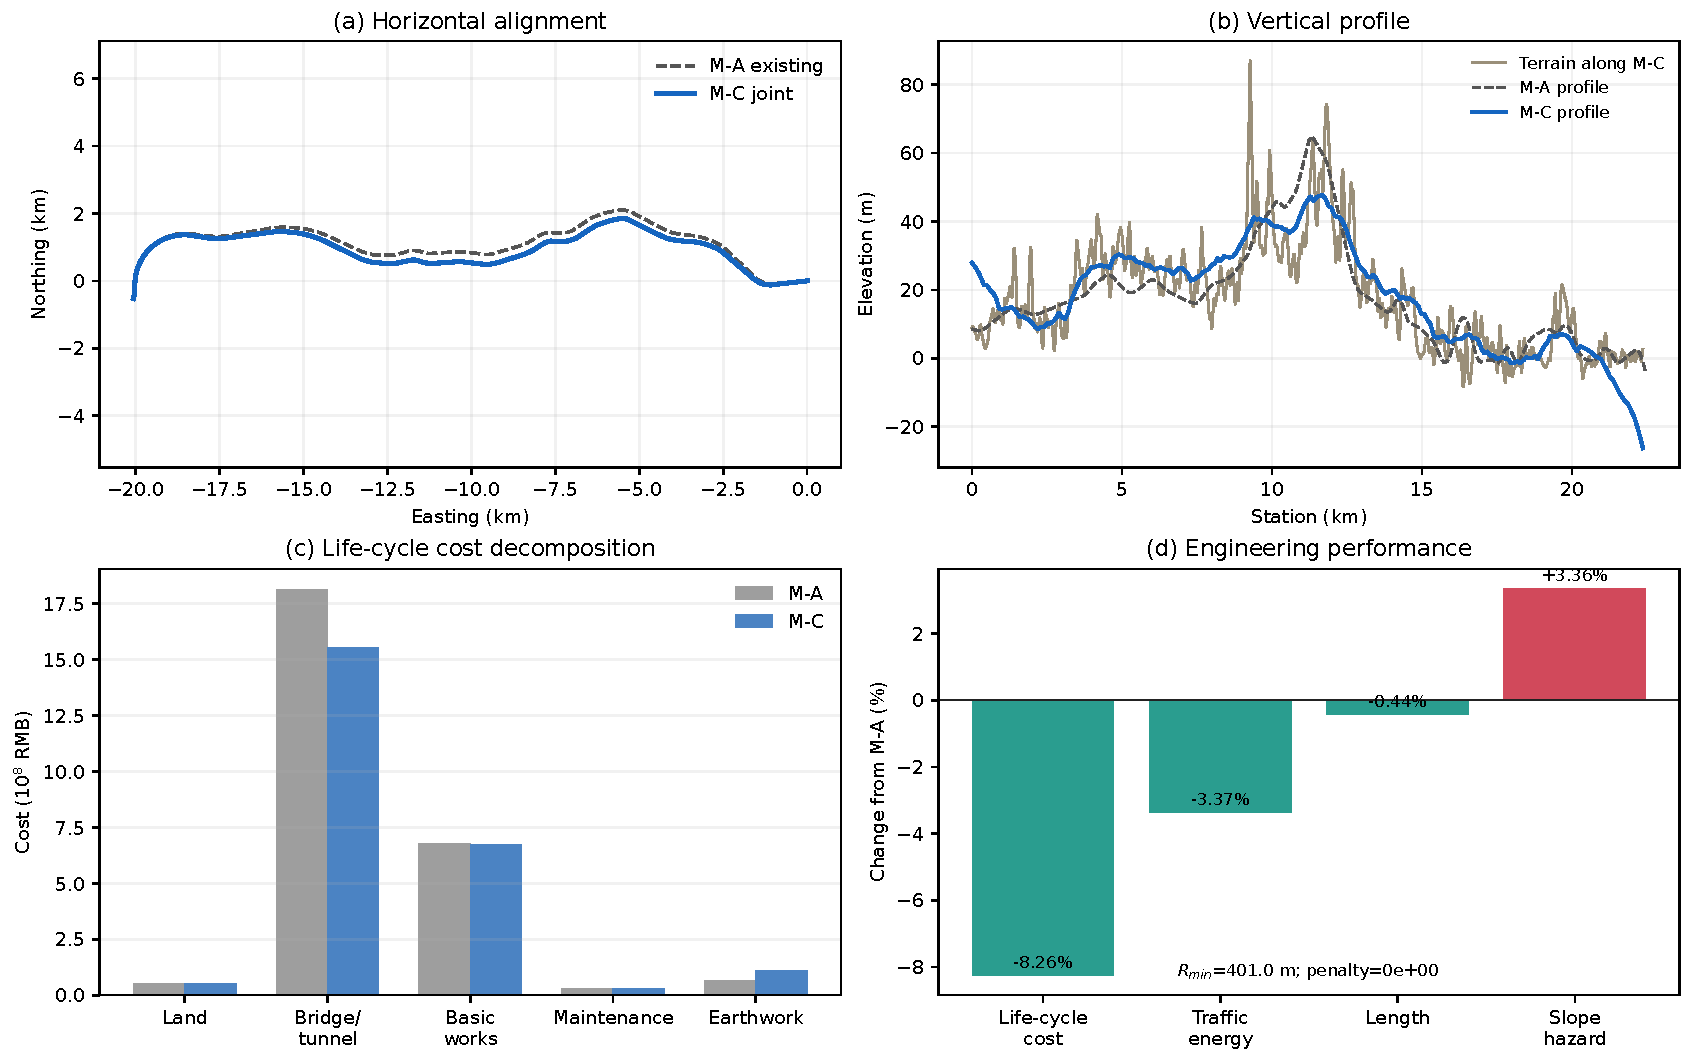
\includegraphics[width=\textwidth]{c132_scheme_summary.pdf}
\caption{固定版本M-A/M-C对比：平面、纵断面、成本分解和主要变化。图中如实显示未锚定的纵断面终点。}
\label{fig:scheme_zh}
\end{figure}

成本机制主要来自结构替代。桥隧费由18.1536亿元降至15.5395亿元，减少2.6141亿元；土方费由0.6717亿元增至1.1267亿元，增加0.4550亿元。占地和基本工程略降，养护费增加0.0088亿元，最终净成本减少2.1822亿元。因此，收益不能仅由98.3 m缩短解释，而是结构费下降与土方增加的综合权衡。

成本—能耗扫描含21个权重搜索。图\ref{fig:pareto_zh}显示可行点和熵权M-C；可行性与10\%预算门槛先剔除不可接受或结构费过高的端点，再计算最终熵权得分。

\begin{figure}[t]
\centering
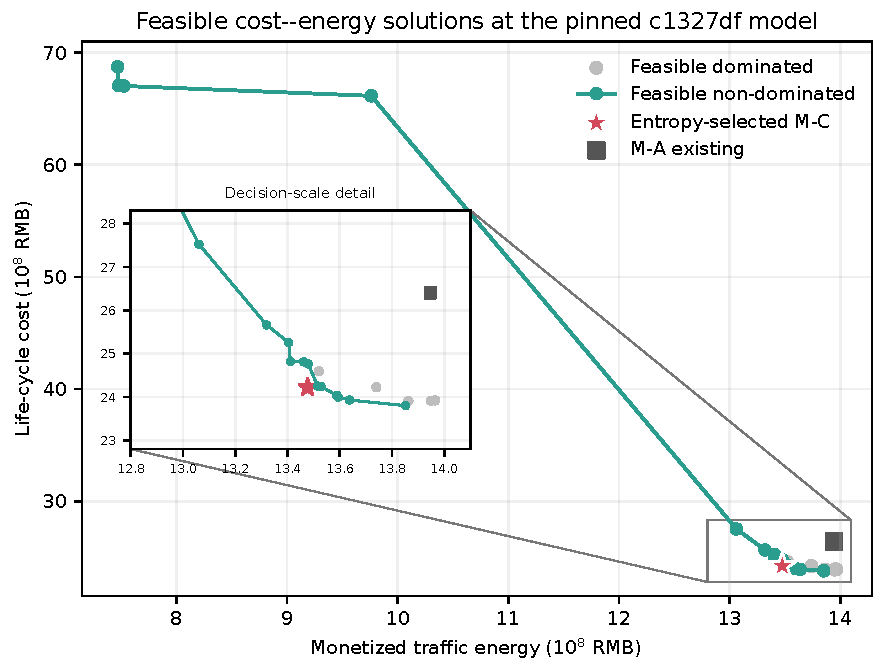
\includegraphics[width=\linewidth]{c132_pareto.pdf}
\caption{固定模型中的可行成本—能耗点与熵权折中方案。}
\label{fig:pareto_zh}
\end{figure}

\subsection{联合优化与两阶段优化}

两阶段对照的原始目标更低，但违反最小半径要求。表\ref{tab:sequential_zh}区分数值目标与工程可接受性：第一阶段平面冻结后，纵断面阶段无法修复397.06 m半径，其罚值保持0.07359。因此，尽管M-C原始成本与能耗略高，可行M-C仍是优选。

\begin{table}[t]
\centering
\caption{共同目标参考下联合与两阶段结果。}
\label{tab:sequential_zh}
\begin{tabular}{lrrr}
\toprule
指标 & M-A & 两阶段 & 联合M-C \\
\midrule
成本（亿元） & 26.4061 & 23.1582 & 24.2239 \\
能耗（亿元） & 13.9460 & 13.4569 & 13.4766 \\
里程（km） & 22.4618 & 22.3659 & 22.3635 \\
$R_{min}$（m） & 422.43 & 397.06 & 401.03 \\
罚值 & 0 & 0.07359 & 0 \\
决策状态 & 可行 & 不可行 & 可行 \\
\bottomrule
\end{tabular}
\end{table}

\subsection{IJS机制消融}\label{sec:ablation_zh}

500代时，完整IJS的观测平均标量目标最低，为0.6808；JS为0.9133，观测差距25.45\%（表\ref{tab:ablation_zh}）。在单算子变体中，JS+DE相对JS的同代数观测差距最大；Tent单独作用的差距较小，且未调整秩和检验不显著。存储收敛记录中，IJS在第187代达到JS最终水平。然而，完整IJS每代也约使用三倍目标评价，因此表格只能说明同代数表现。

\begin{table}[t]
\centering
\caption{30次纵断面测试床消融。$p$值为未调整独立样本秩和检验，NFE因变体而异。}
\label{tab:ablation_zh}
\begin{tabular}{lrrrrr}
\toprule
变体 & 平均$F$ & 标准差 & $F_{100}$ & 相对JS差距 & $p$ \\
\midrule
JS & 0.9133 & 0.0637 & 2.547 & -- & -- \\
JS+Tent & 0.8989 & 0.0605 & 2.227 & 1.58\% & 0.464 \\
JS+L\'evy & 0.8787 & 0.0558 & 2.095 & 3.79\% & 0.0555 \\
JS+DE & 0.6926 & 0.0315 & 1.679 & 24.17\% & $3.02\times10^{-11}$ \\
IJS & \textbf{0.6808} & 0.0340 & \textbf{1.292} & \textbf{25.45\%} & $3.02\times10^{-11}$ \\
\bottomrule
\end{tabular}
\end{table}

\subsection{多算法对比}

六种分辨率下IJS均取得最低存储平均$F$（表\ref{tab:benchmark_zh}）。PJ6中IJS与JS的10次运行全部可行，其他四种方法返回罚值主导解。IJS在PJ1--PJ5的耗时约为JS的1.9倍，在PJ6约为2.8倍，同时还执行更多目标调用。因此，合理结论是该多阶段实现在本记录中取得最低同代数目标和更强的高分辨率可行性，而不是等预算下已经证明优越。

\begin{table*}[t]
\centering
\caption{10次运行目标均值（标准差）。相同代数不等于相同NFE。}
\label{tab:benchmark_zh}
\scriptsize
\resizebox{\textwidth}{!}{\begin{tabular}{lrrrrrr}
\toprule
算法 & PJ1（95） & PJ2 & PJ3 & PJ4 & PJ5 & PJ6（500） \\
\midrule
IJS & \textbf{.6617 (.0051)} & \textbf{.5986 (.0045)} & \textbf{.7087 (.0045)} & \textbf{.7090 (.0033)} & \textbf{.7778 (.0078)} & \textbf{.8333 (.0019)} \\
JS & .6771 (.0052) & .6104 (.0049) & .7237 (.0063) & .7215 (.0066) & .7954 (.0020) & .8563 (.0060) \\
NSGA-II & .6792 (.0045) & .6240 (.0057) & .7282 (.0053) & .7287 (.0080) & .8104 (.0084) & 12.8859 (.7330) \\
GA & .7103 (.0088) & .6478 (.0171) & .7515 (.0090) & .7489 (.0071) & 5.3906 (.5481) & 25.6024 (1.0630) \\
PSO & .7023 (.0116) & .6370 (.0113) & .7436 (.0070) & .7632 (.0072) & 9.1988 (.9109) & 32.7437 (.6336) \\
GWO & .6843 (.0065) & .6194 (.0070) & .7233 (.0046) & .7276 (.0070) & 1.1104 (.0158) & 3.2157 (1.5706) \\
\bottomrule
\end{tabular}}
\end{table*}

\subsection{固定模型族敏感性}

存储的237次敏感性重优化均被其实现检查标记为可行。交通增长对货币化能耗响应最强；成本对需求、车队与能源价格较不敏感，因为基础设施支出主要发生在建设期。电动车比例提高可缓和高需求下的能源负担，油电价格同步增长则提高$E$。

谱宽响应先强后趋缓：$W=200$ m时优化成本为25.68亿元，$W=2{,}500$ m时为22.39亿元。这支持把$W$解释为搜索灵活度而非硬走廊半宽。$E_{ext}=50/75/100$ m时成本分别为22.81/23.55/24.74亿元，而能耗保持约13.55亿元，说明桥梁延伸假设会显著影响经济结果。

\begin{figure}[!htbp]
\centering
\begin{subfigure}{.78\textwidth}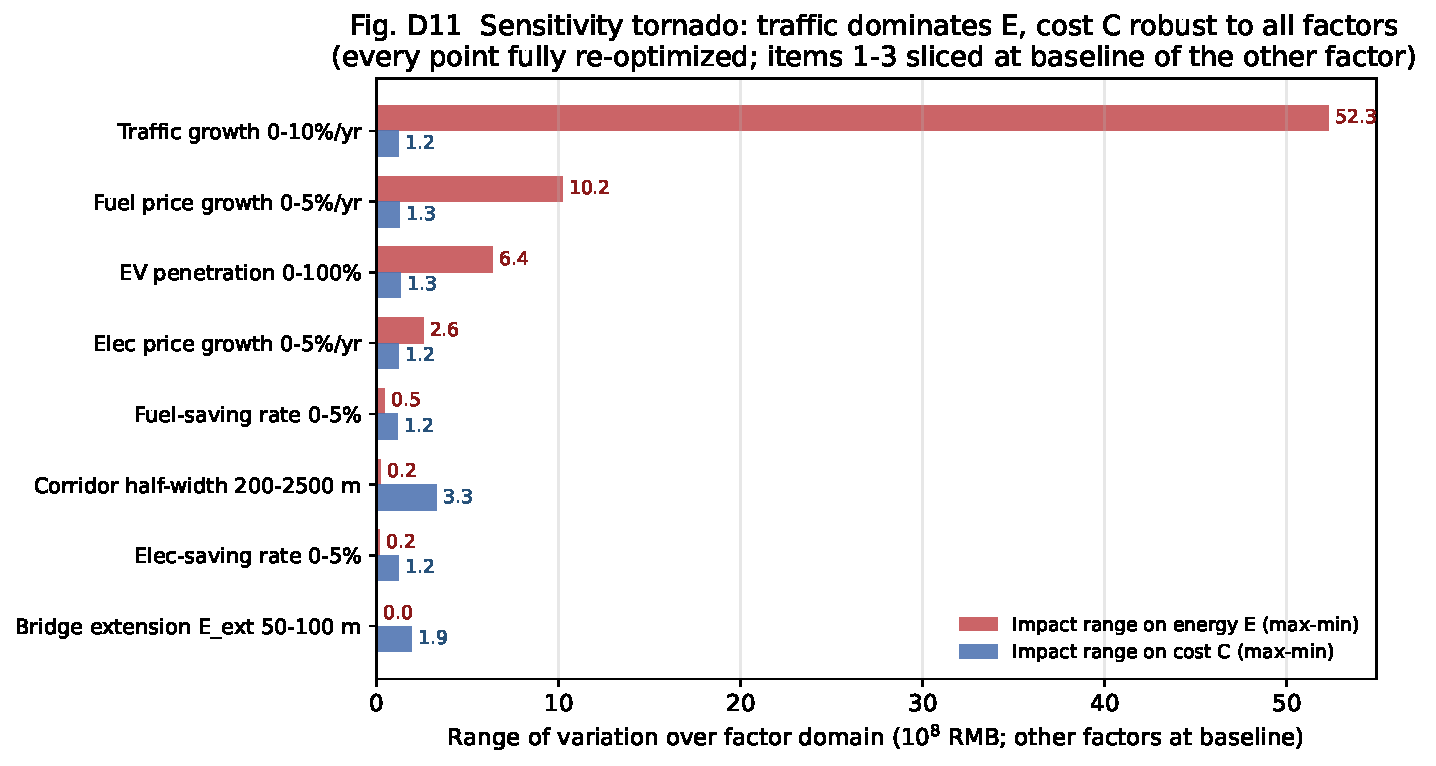
\includegraphics[width=\linewidth]{sensitivity_tornado.pdf}\caption{运行情景相对重要性。}\end{subfigure}\\[3mm]
\begin{subfigure}{.78\textwidth}
\includegraphics[width=\linewidth]{corridor_sensitivity.pdf}\caption{谱宽$W$重优化。}\end{subfigure}
\caption{固定提交中已经存在的敏感性结果。}
\label{fig:sensitivity_zh}
\end{figure}
\FloatBarrier

\section{讨论}

\subsection{工程含义}

8.26\%和3.37\%是共同数据与单价下的案例模型变化，不能外推为普遍节省率。其价值在于分项可追踪：M-C缩短0.44\%，但2.6141亿元结构费减少远大于98.3 m长度本身能够解释的成本；优化器以更多土方和略高边坡危险度诊断换取较低结构暴露与运行能耗。

两阶段对照说明可行性必须先于目标大小。其397.06 m最小半径违反400 m阈值，因此更低$C$与$E$不能被解释为更优工程方案。联合搜索在约束边界附近同时保留调整平面和纵断面的能力；固定记录显示联合方案可行，而本次两阶段方案不可行。

\subsection{空间数据与算法作用}

候选特定DEM采样使平面横移真正改变地面，而不只是改变长度。OSM相交把位置转化为桥梁需求，连通山体掩膜使生态隧道长度内生。这些机制提高了可审计性，但仍是规划抽象：OSM缺少可靠桥面高程和地块属性，重建DEM也不是测量级施工前地表。

Tent、L\'evy和DE分别具有覆盖、探索和细化的合理作用。在单算子变体中，JS+DE相对JS的同代数观测差距最大；该结果不能分离出按评价预算归一化后的DE效应。故算法证据支持当前实现流程并提出等NFE研究假设，却不能隔离出固有25.45\%优势。

\subsection{局限性与效度边界}\label{sec:limitations_zh}

\begin{enumerate}[leftmargin=*,label=(\arabic*)]
\item 纵断面起终点自由。所选M-C终点高程在图中明显低于现状端点，会同时影响土方与单向能耗；8.26\%/3.37\%不能表述为固定接线设计结果。
\item 能耗只评价一个代表方向。最终设计需要双向交通加权和经标定的再生制动模型，以消除净高差敏感性。
\item 相邻坡差只是竖曲线代理，尚缺凸/凹竖曲线半径与长度、视距、缓和曲线/圆曲线分段及完整平纵协调检查。
\item 准天然DEM由既有道路表面重建，分辨率约8.8 m；OSM覆盖和交叉分类不均，障碍物竖向净空未经验证。
\item 固定模型没有建筑密度约束，概念图中的城市绕避不能解释为已计算约束或收益。
\item 成本单价属于规划估计；地质、水文、征地拆迁、施工组织、隐含碳和不确定性需要项目数据。
\item 工程方案为单次优化。消融和算法比较采用相同代数但NFE不等，秩和检验未经多重校正，因此尚未确认等预算算法优势。
\end{enumerate}

因此，本框架提供可审计的走廊规划证据和可复现计算案例，不能替代详细几何设计，也不能支持普遍节省率。

\section{结论}

本文将候选三维高速公路线形与准天然地形、OSM触发结构、全生命周期成本及油电混行车流能耗联系起来。275变量平纵协同表示由IJS搜索，并在熵权折中前执行可行性、预算和非支配筛选。

在固定\texttt{c1327df}版本中，广州北环联合方案成本下降8.26\%、货币化能耗下降3.37\%、里程缩短0.44\%，以$R_{min}=401.03$ m和零罚值满足半径要求。主要经济机制是结构费减少2.6141亿元，超过土方增加0.4550亿元。原始目标更低的两阶段方案因半径397.06 m而被否决。IJS在存储消融和算法对比中取得最低同代数观测目标，但NFE不等使其不能证明等预算优势。

下一步最重要的模型修正是固定纵断面两端并评价双向交通，之后才能把线位解释为设计级方案。等NFE多种子算法比较、显式竖曲线和测量/地块数据同样必要。这些属于局限性和未来工作，不是用于改变本文结果的补充实验。

\section*{数据与代码可用性}
全文数值及论文专用图严格绑定Git提交\texttt{c1327df}，完整哈希记录于源文件清单。草稿包包含源值快照、SHA-256清单和仅从不可变Git对象读取数据的制图脚本，不会执行优化器。GNSS及项目派生数据可能受所有者限制；匿名审查后应补充公开仓库DOI。

\section*{作者贡献}
\textbf{[作者占位]}：概念设计、方法、软件、验证、调查、数据整理、可视化、初稿、审阅与修改。投稿前按真实分工替换。

\section*{利益冲突声明}
作者声明不存在可能影响本文工作的已知经济利益或个人关系；投稿前须由全部作者确认。

\section*{致谢}
基金名称、编号及非作者贡献因双盲审稿暂作匿名占位，投稿前补全。

\bibliographystyle{elsarticle-num}
\bibliography{../references}

\end{document}
